\documentclass{beamer}
\usepackage[T1]{fontenc}
\usepackage[utf8]{inputenc}
\usepackage{lmodern}
\usepackage[english]{babel}

\usepackage{verbatim}
\usepackage{mathtools}
\usepackage{stmaryrd}


\usepackage{geometry}
\usepackage{setspace}

\usepackage{latex/agda}
\usepackage{unicode-math}
\setmathfont{XITS Math}

\usepackage{newunicodechar}
\newunicodechar{→}{\ensuremath{\mathnormal\to}}
\newunicodechar{ℕ}{\ensuremath{\mathnormal\bN}}
\newunicodechar{ℓ}{\ensuremath{\mathnormal\ell}}
\newunicodechar{↪}{\ensuremath{\mathnormal\hookrightarrow}}
\newunicodechar{𝑀}{$M$}

% \newunicodechar{ℕ}{$\mathbb{N}$}
\newunicodechar{⊨}{\ensuremath{\vDash}}
\newunicodechar{⊧}{$\models$}

\newunicodechar{ϕ}{$\phi$}
\newunicodechar{∨}{$\lor$}
\newunicodechar{∧}{$\land$}
\newunicodechar{⇒}{$\Rightarrow$}

\newunicodechar{⊥}{$\bot$}
\newunicodechar{⊤}{$\top$}
% ⊥ ⊤
  % _∨_ _∧_ _⇒_ : → ϕ → ϕ


\usepackage{xcolor}
\usepackage[normalem]{ulem}%per barrare parole
\usepackage{soul} %barrare numeri
% \usepackage{booktabs}%per tabelle
\usepackage{amsmath} %leqno mette elenchi in align a sx
\usepackage{amssymb}
% \usepackage{enumitem} %personalizza gli elenchi
% \usepackage{amsthm} %teoremi e definizioni
\usepackage{tikz-cd}
% \tikzcdset{scale cd/.style={every label/.append style={scale=#1} }}
\tikzcdset{scale cd/.style={every label/.append style={scale=#1}, cells={nodes={scale=#1}}}}

\usepackage{multirow}%più righe nella stessa cella in tabella
\usepackage{multicol}
\usepackage{caption}
\usepackage{bussproofs}
\usepackage{soul}
\newcommand{\mathcolorbox}[2]{\colorbox{#1}{$\displaystyle #2$}}

\usetheme{Antibes}
\usecolortheme{beaver}
\useinnertheme{rounded}
\useoutertheme{infolines}

\titlegraphic{
  
\includegraphics[width=25mm]{pics/hw.png}
  
\includegraphics[width=25mm]{pics/aisec.png}
  
\includegraphics[width=25mm]{pics/laiv.png}}
\title{On the syntax and semantics of voice assistants in autonomous vehicles}
\author{Warrick Macmillan}
\date{$6^{th}$ May 2022}



\begin{document}

\begin{frame}
  \titlepage
\end{frame}

\section{Overview}


% \subsection{Quick Recapitulation}

\begin{frame}
\begin{code}[hide]%
\>[0]\AgdaKeyword{module}\AgdaSpace{}%
\AgdaModule{Syntax}\AgdaSpace{}%
\AgdaSymbol{(}\AgdaBound{Atom}\AgdaSpace{}%
\AgdaSymbol{:}\AgdaSpace{}%
\AgdaPrimitive{Set}\AgdaSymbol{)}\AgdaSpace{}%
\AgdaKeyword{where}\<%
\\
\>[0]\AgdaComment{-- Think Atom =FinSet}\<%
\end{code}
\begin{code}%
\>[0]\AgdaKeyword{data}\AgdaSpace{}%
\AgdaDatatype{ϕ}\AgdaSpace{}%
\AgdaSymbol{:}\AgdaSpace{}%
\AgdaPrimitive{Set}\AgdaSpace{}%
\AgdaKeyword{where}\<%
\\
\>[0][@{}l@{\AgdaIndent{0}}]%
\>[2]\AgdaInductiveConstructor{atom}%
\>[14]\AgdaSymbol{:}\AgdaSpace{}%
\AgdaBound{Atom}\AgdaSpace{}%
\AgdaSymbol{→}\AgdaSpace{}%
\AgdaDatatype{ϕ}\<%
\\
%
\>[2]\AgdaInductiveConstructor{⊥}\AgdaSpace{}%
\AgdaInductiveConstructor{⊤}%
\>[14]\AgdaSymbol{:}\AgdaSpace{}%
\AgdaDatatype{ϕ}\<%
\\
%
\>[2]\AgdaOperator{\AgdaInductiveConstructor{¬\AgdaUnderscore{}}}%
\>[14]\AgdaSymbol{:}\AgdaSpace{}%
\AgdaDatatype{ϕ}\AgdaSpace{}%
\AgdaSymbol{→}\AgdaSpace{}%
\AgdaDatatype{ϕ}\<%
\\
%
\>[2]\AgdaOperator{\AgdaInductiveConstructor{\AgdaUnderscore{}∨\AgdaUnderscore{}}}\AgdaSpace{}%
\AgdaOperator{\AgdaInductiveConstructor{\AgdaUnderscore{}∧\AgdaUnderscore{}}}\AgdaSpace{}%
\AgdaOperator{\AgdaInductiveConstructor{\AgdaUnderscore{}⇒\AgdaUnderscore{}}}\AgdaSpace{}%
\AgdaSymbol{:}\AgdaSpace{}%
\AgdaDatatype{ϕ}\AgdaSpace{}%
\AgdaSymbol{→}\AgdaSpace{}%
\AgdaDatatype{ϕ}\AgdaSpace{}%
\AgdaSymbol{→}\AgdaSpace{}%
\AgdaDatatype{ϕ}\<%
\\
%
\>[2]\AgdaInductiveConstructor{X}\AgdaSpace{}%
\AgdaInductiveConstructor{F}\AgdaSpace{}%
\AgdaInductiveConstructor{G}%
\>[14]\AgdaSymbol{:}\AgdaSpace{}%
\AgdaDatatype{ϕ}\AgdaSpace{}%
\AgdaSymbol{→}\AgdaSpace{}%
\AgdaDatatype{ϕ}\<%
\\
%
\>[2]\AgdaOperator{\AgdaInductiveConstructor{\AgdaUnderscore{}U\AgdaUnderscore{}}}\AgdaSpace{}%
\AgdaOperator{\AgdaInductiveConstructor{\AgdaUnderscore{}W\AgdaUnderscore{}}}\AgdaSpace{}%
\AgdaOperator{\AgdaInductiveConstructor{\AgdaUnderscore{}R\AgdaUnderscore{}}}\AgdaSpace{}%
\AgdaSymbol{:}\AgdaSpace{}%
\AgdaDatatype{ϕ}\AgdaSpace{}%
\AgdaSymbol{→}\AgdaSpace{}%
\AgdaDatatype{ϕ}\AgdaSpace{}%
\AgdaSymbol{→}\AgdaSpace{}%
\AgdaDatatype{ϕ}\<%
\end{code}
\begin{code}[hide]%
\>[0]\AgdaKeyword{open}\AgdaSpace{}%
\AgdaKeyword{import}\AgdaSpace{}%
\AgdaModule{Data.List}\<%
\\
%
\\[\AgdaEmptyExtraSkip]%
\>[0]\AgdaComment{-- that it automatically satisfies true, so if there are no location propositions}\<%
\\
\>[0]\AgdaComment{-- a trace is just a list of atoms}\<%
\\
\>[0]\AgdaComment{-- coverage versus surveillance patterns}\<%
\\
%
\\[\AgdaEmptyExtraSkip]%
\>[0]\AgdaComment{-- data atoms : Set where}\<%
\\
\>[0]\AgdaComment{--   corner : atoms}\<%
\\
\>[0]\AgdaComment{--   person : atoms}\<%
\\
\>[0]\AgdaComment{--   home   : atoms}\<%
\\
\>[0]\AgdaComment{--   cafe   : atoms}\<%
\\
%
\\[\AgdaEmptyExtraSkip]%
\>[0]\AgdaComment{--eventually visit all the ls}\<%
\\
\>[0]\AgdaFunction{visit}\AgdaSpace{}%
\AgdaSymbol{:}\AgdaSpace{}%
\AgdaDatatype{List}\AgdaSpace{}%
\AgdaBound{Atom}\AgdaSpace{}%
\AgdaSymbol{→}\AgdaSpace{}%
\AgdaDatatype{ϕ}\<%
\\
\>[0]\AgdaFunction{visit}\AgdaSpace{}%
\AgdaInductiveConstructor{[]}\AgdaSpace{}%
\AgdaSymbol{=}\AgdaSpace{}%
\AgdaInductiveConstructor{⊤}\<%
\\
\>[0]\AgdaFunction{visit}\AgdaSpace{}%
\AgdaSymbol{(}\AgdaBound{l}\AgdaSpace{}%
\AgdaOperator{\AgdaInductiveConstructor{∷}}\AgdaSpace{}%
\AgdaBound{ls}\AgdaSymbol{)}\AgdaSpace{}%
\AgdaSymbol{=}\AgdaSpace{}%
\AgdaSymbol{(}\AgdaInductiveConstructor{F}\AgdaSpace{}%
\AgdaSymbol{(}\AgdaInductiveConstructor{atom}\AgdaSpace{}%
\AgdaBound{l}\AgdaSymbol{))}\AgdaSpace{}%
\AgdaOperator{\AgdaInductiveConstructor{∧}}\AgdaSpace{}%
\AgdaFunction{visit}\AgdaSpace{}%
\AgdaBound{ls}\<%
\\
%
\\[\AgdaEmptyExtraSkip]%
\>[0]\AgdaComment{-- eventually replace eventually with efficiently : (i.e. minimize energy such that you get there)}\<%
\\
%
\\[\AgdaEmptyExtraSkip]%
\>[0]\AgdaComment{--eventually visit l1, and then eventually visit l2,}\<%
\\
\>[0]\AgdaFunction{sequentialVisit}\AgdaSpace{}%
\AgdaSymbol{:}\AgdaSpace{}%
\AgdaDatatype{List}\AgdaSpace{}%
\AgdaBound{Atom}\AgdaSpace{}%
\AgdaSymbol{→}\AgdaSpace{}%
\AgdaDatatype{ϕ}\<%
\\
\>[0]\AgdaFunction{sequentialVisit}\AgdaSpace{}%
\AgdaInductiveConstructor{[]}\AgdaSpace{}%
\AgdaSymbol{=}\AgdaSpace{}%
\AgdaInductiveConstructor{⊤}\<%
\\
\>[0]\AgdaFunction{sequentialVisit}\AgdaSpace{}%
\AgdaSymbol{(}\AgdaBound{l}\AgdaSpace{}%
\AgdaOperator{\AgdaInductiveConstructor{∷}}\AgdaSpace{}%
\AgdaBound{ls}\AgdaSymbol{)}\AgdaSpace{}%
\AgdaSymbol{=}\AgdaSpace{}%
\AgdaInductiveConstructor{F}\AgdaSpace{}%
\AgdaSymbol{(}\AgdaInductiveConstructor{atom}\AgdaSpace{}%
\AgdaBound{l}\AgdaSpace{}%
\AgdaOperator{\AgdaInductiveConstructor{∧}}\AgdaSpace{}%
\AgdaFunction{sequentialVisit}\AgdaSpace{}%
\AgdaBound{ls}\AgdaSymbol{)}\<%
\\
%
\\[\AgdaEmptyExtraSkip]%
\>[0]\AgdaComment{-- suppose the driver doesn't actually care if they visit all the locations, as}\<%
\\
\>[0]\AgdaComment{-- long as they get to the last location}\<%
\\
\>[0]\AgdaFunction{weakSequentialVisit}\AgdaSpace{}%
\AgdaSymbol{:}\AgdaSpace{}%
\AgdaDatatype{List}\AgdaSpace{}%
\AgdaBound{Atom}\AgdaSpace{}%
\AgdaSymbol{→}\AgdaSpace{}%
\AgdaDatatype{ϕ}\<%
\\
\>[0]\AgdaFunction{weakSequentialVisit}\AgdaSpace{}%
\AgdaInductiveConstructor{[]}\AgdaSpace{}%
\AgdaSymbol{=}\AgdaSpace{}%
\AgdaInductiveConstructor{⊤}\<%
\\
\>[0]\AgdaFunction{weakSequentialVisit}\AgdaSpace{}%
\AgdaBound{lss}\AgdaSymbol{@(}\AgdaBound{l}\AgdaSpace{}%
\AgdaOperator{\AgdaInductiveConstructor{∷}}\AgdaSpace{}%
\AgdaBound{ls}\AgdaSymbol{)}\AgdaSpace{}%
\AgdaSymbol{=}\AgdaSpace{}%
\AgdaFunction{sequentialVisit}\AgdaSpace{}%
\AgdaBound{lss}\AgdaSpace{}%
\AgdaOperator{\AgdaInductiveConstructor{∨}}\AgdaSpace{}%
\AgdaFunction{weakSequentialVisit}\AgdaSpace{}%
\AgdaBound{ls}\<%
\\
%
\\[\AgdaEmptyExtraSkip]%
\>[0]\AgdaComment{-- ordering condition}\<%
\\
\>[0]\AgdaComment{-- don't visit li+1 until you've visited li}\<%
\\
\>[0]\AgdaFunction{predecessorPrecedesSuccessor}\AgdaSpace{}%
\AgdaSymbol{:}\AgdaSpace{}%
\AgdaDatatype{List}\AgdaSpace{}%
\AgdaBound{Atom}\AgdaSpace{}%
\AgdaSymbol{→}\AgdaSpace{}%
\AgdaDatatype{ϕ}\<%
\\
\>[0]\AgdaFunction{predecessorPrecedesSuccessor}\AgdaSpace{}%
\AgdaInductiveConstructor{[]}\AgdaSpace{}%
\AgdaSymbol{=}\AgdaSpace{}%
\AgdaInductiveConstructor{⊤}\<%
\\
\>[0]\AgdaFunction{predecessorPrecedesSuccessor}\AgdaSpace{}%
\AgdaSymbol{(}\AgdaBound{l}\AgdaSpace{}%
\AgdaOperator{\AgdaInductiveConstructor{∷}}\AgdaSpace{}%
\AgdaInductiveConstructor{[]}\AgdaSymbol{)}\AgdaSpace{}%
\AgdaSymbol{=}\AgdaSpace{}%
\AgdaInductiveConstructor{⊤}\<%
\\
\>[0]\AgdaFunction{predecessorPrecedesSuccessor}\AgdaSpace{}%
\AgdaSymbol{(}\AgdaBound{lᵢ}\AgdaSpace{}%
\AgdaOperator{\AgdaInductiveConstructor{∷}}\AgdaSpace{}%
\AgdaBound{lᵢ₊₁}\AgdaSpace{}%
\AgdaOperator{\AgdaInductiveConstructor{∷}}\AgdaSpace{}%
\AgdaBound{ls}\AgdaSymbol{)}\AgdaSpace{}%
\AgdaSymbol{=}\<%
\\
\>[0][@{}l@{\AgdaIndent{0}}]%
\>[2]\AgdaSymbol{((}\AgdaOperator{\AgdaInductiveConstructor{¬}}\AgdaSpace{}%
\AgdaInductiveConstructor{atom}\AgdaSpace{}%
\AgdaBound{lᵢ₊₁}\AgdaSymbol{)}\AgdaSpace{}%
\AgdaOperator{\AgdaInductiveConstructor{U}}\AgdaSpace{}%
\AgdaInductiveConstructor{atom}\AgdaSpace{}%
\AgdaBound{lᵢ}\AgdaSymbol{)}\AgdaSpace{}%
\AgdaOperator{\AgdaInductiveConstructor{∧}}\AgdaSpace{}%
\AgdaFunction{predecessorPrecedesSuccessor}\AgdaSpace{}%
\AgdaSymbol{(}\AgdaBound{lᵢ₊₁}\AgdaSpace{}%
\AgdaOperator{\AgdaInductiveConstructor{∷}}\AgdaSpace{}%
\AgdaBound{ls}\AgdaSymbol{)}\<%
\\
%
\\[\AgdaEmptyExtraSkip]%
\>[0]\AgdaFunction{orderedVisit}\AgdaSpace{}%
\AgdaSymbol{:}\AgdaSpace{}%
\AgdaDatatype{List}\AgdaSpace{}%
\AgdaBound{Atom}\AgdaSpace{}%
\AgdaSymbol{→}\AgdaSpace{}%
\AgdaDatatype{ϕ}\<%
\\
\>[0]\AgdaFunction{orderedVisit}\AgdaSpace{}%
\AgdaBound{ls}\AgdaSpace{}%
\AgdaSymbol{=}\AgdaSpace{}%
\AgdaFunction{sequentialVisit}\AgdaSpace{}%
\AgdaBound{ls}\AgdaSpace{}%
\AgdaOperator{\AgdaInductiveConstructor{∧}}\AgdaSpace{}%
\AgdaFunction{predecessorPrecedesSuccessor}\AgdaSpace{}%
\AgdaBound{ls}\<%
\\
%
\\[\AgdaEmptyExtraSkip]%
\>[0]\AgdaComment{-- strictness condition}\<%
\\
\>[0]\AgdaComment{-- don't visit a location twice}\<%
\\
\>[0]\AgdaComment{-- probably not realistic for our example}\<%
\\
\>[0]\AgdaComment{-- everything should also depend on the location of the vehicle}\<%
\\
\>[0]\AgdaComment{-- past temporal operators should be used to judge the success of a mission}\<%
\\
\>[0]\AgdaFunction{strictSeq}\AgdaSpace{}%
\AgdaSymbol{:}\AgdaSpace{}%
\AgdaDatatype{List}\AgdaSpace{}%
\AgdaBound{Atom}\AgdaSpace{}%
\AgdaSymbol{→}\AgdaSpace{}%
\AgdaDatatype{ϕ}\<%
\\
\>[0]\AgdaFunction{strictSeq}\AgdaSpace{}%
\AgdaInductiveConstructor{[]}\AgdaSpace{}%
\AgdaSymbol{=}\AgdaSpace{}%
\AgdaInductiveConstructor{⊤}\<%
\\
\>[0]\AgdaFunction{strictSeq}\AgdaSpace{}%
\AgdaSymbol{(}\AgdaBound{l}\AgdaSpace{}%
\AgdaOperator{\AgdaInductiveConstructor{∷}}\AgdaSpace{}%
\AgdaInductiveConstructor{[]}\AgdaSymbol{)}\AgdaSpace{}%
\AgdaSymbol{=}\AgdaSpace{}%
\AgdaInductiveConstructor{⊤}\<%
\\
\>[0]\AgdaFunction{strictSeq}\AgdaSpace{}%
\AgdaSymbol{(}\AgdaBound{lᵢ}\AgdaSpace{}%
\AgdaOperator{\AgdaInductiveConstructor{∷}}\AgdaSpace{}%
\AgdaBound{lᵢ₊₁}\AgdaSpace{}%
\AgdaOperator{\AgdaInductiveConstructor{∷}}\AgdaSpace{}%
\AgdaBound{ls}\AgdaSymbol{)}\AgdaSpace{}%
\AgdaSymbol{=}\AgdaSpace{}%
\AgdaSymbol{((}\AgdaOperator{\AgdaInductiveConstructor{¬}}\AgdaSpace{}%
\AgdaInductiveConstructor{atom}\AgdaSpace{}%
\AgdaBound{lᵢ₊₁}\AgdaSymbol{)}\AgdaSpace{}%
\AgdaOperator{\AgdaInductiveConstructor{U}}\AgdaSpace{}%
\AgdaSymbol{(}\AgdaInductiveConstructor{atom}\AgdaSpace{}%
\AgdaBound{lᵢ}\AgdaSpace{}%
\AgdaOperator{\AgdaInductiveConstructor{∧}}\AgdaSpace{}%
\AgdaInductiveConstructor{X}\AgdaSpace{}%
\AgdaSymbol{((}\AgdaOperator{\AgdaInductiveConstructor{¬}}\AgdaSpace{}%
\AgdaInductiveConstructor{atom}\AgdaSpace{}%
\AgdaBound{lᵢ}\AgdaSymbol{)}\AgdaSpace{}%
\AgdaOperator{\AgdaInductiveConstructor{U}}\AgdaSpace{}%
\AgdaInductiveConstructor{atom}\AgdaSpace{}%
\AgdaBound{lᵢ₊₁}\AgdaSymbol{)))}\AgdaSpace{}%
\AgdaOperator{\AgdaInductiveConstructor{∧}}\AgdaSpace{}%
\AgdaFunction{strictSeq}\AgdaSpace{}%
\AgdaSymbol{(}\AgdaBound{lᵢ₊₁}\AgdaSpace{}%
\AgdaOperator{\AgdaInductiveConstructor{∷}}\AgdaSpace{}%
\AgdaBound{ls}\AgdaSymbol{)}\<%
\\
%
\\[\AgdaEmptyExtraSkip]%
\>[0]\AgdaFunction{strictOrderedVisit}\AgdaSpace{}%
\AgdaSymbol{:}\AgdaSpace{}%
\AgdaDatatype{List}\AgdaSpace{}%
\AgdaBound{Atom}\AgdaSpace{}%
\AgdaSymbol{→}\AgdaSpace{}%
\AgdaDatatype{ϕ}\<%
\\
\>[0]\AgdaFunction{strictOrderedVisit}\AgdaSpace{}%
\AgdaBound{ls}\AgdaSpace{}%
\AgdaSymbol{=}\AgdaSpace{}%
\AgdaFunction{orderedVisit}\AgdaSpace{}%
\AgdaBound{ls}\AgdaSpace{}%
\AgdaOperator{\AgdaInductiveConstructor{∧}}\AgdaSpace{}%
\AgdaFunction{strictSeq}\AgdaSpace{}%
\AgdaBound{ls}\<%
\\
%
\\[\AgdaEmptyExtraSkip]%
\>[0]\AgdaComment{-- define a satisfaction for a trace -- only care about the finite case, but really we should generalize this}\<%
\\
\>[0]\AgdaComment{-- can ask if a trace satisisfies a formula}\<%
\\
%
\\[\AgdaEmptyExtraSkip]%
\>[0]\AgdaComment{--Mission specifications}\<%
\\
\>[0]\AgdaComment{-- are used, among others, to synthesize, verify, simulate or guide}\<%
\\
\>[0]\AgdaComment{-- the engineering of robot software}\<%
\\
%
\\[\AgdaEmptyExtraSkip]%
\>[0]\AgdaComment{--fair visit and patrolling, could be interpreted with respect to taking the cab around}\<%
\\
\>[0]\AgdaComment{-- a trace is just a path where the labeller is restricted to singleton sets}\<%
\\
%
\\[\AgdaEmptyExtraSkip]%
\>[0]\AgdaComment{-- G (isRed -> (break U vel == 0) U isGreen) (unless there is an ambulance)}\<%
\\
%
\\[\AgdaEmptyExtraSkip]%
\>[0]\AgdaComment{-- stop is really a slow and stay stop}\<%
\\
%
\\[\AgdaEmptyExtraSkip]%
\>[0]\AgdaComment{-- G (isGreen -> Go)}\<%
\\
%
\\[\AgdaEmptyExtraSkip]%
\>[0]\AgdaComment{-- globally, obey}\<%
\end{code}

\end{frame}

% \begin{frame}
% \begin{code}%
\>[0]\<%
\\
\>[0]\AgdaKeyword{open}\AgdaSpace{}%
\AgdaKeyword{import}\AgdaSpace{}%
\AgdaModule{F}\<%
\\
%
\\[\AgdaEmptyExtraSkip]%
\>[0]\AgdaFunction{plus}\AgdaSpace{}%
\AgdaSymbol{:}\AgdaSpace{}%
\AgdaDatatype{Nat}\AgdaSpace{}%
\AgdaSymbol{→}\AgdaSpace{}%
\AgdaDatatype{Nat}\AgdaSpace{}%
\AgdaSymbol{→}\AgdaSpace{}%
\AgdaDatatype{Nat}\<%
\\
\>[0]\AgdaFunction{plus}\AgdaSpace{}%
\AgdaInductiveConstructor{zero}\AgdaSpace{}%
\AgdaBound{b}\AgdaSpace{}%
\AgdaSymbol{=}\AgdaSpace{}%
\AgdaBound{b}\<%
\\
\>[0]\AgdaFunction{plus}\AgdaSpace{}%
\AgdaSymbol{(}\AgdaInductiveConstructor{suc}\AgdaSpace{}%
\AgdaBound{a}\AgdaSymbol{)}\AgdaSpace{}%
\AgdaBound{b}\AgdaSpace{}%
\AgdaSymbol{=}\AgdaSpace{}%
\AgdaInductiveConstructor{suc}\AgdaSpace{}%
\AgdaSymbol{(}\AgdaFunction{plus}\AgdaSpace{}%
\AgdaBound{a}\AgdaSpace{}%
\AgdaBound{b}\AgdaSymbol{)}\<%
\\
\>[0]\<%
\end{code}

% \end{frame}



\begin{frame}
\frametitle{Motivation}

\begin{exampleblock}{}

  ``Go to the grocery store after the next exit, and then go to fuel station,
but stop by the fire hydrant so I can take a picture of that crazy sign,
first.''

\end{exampleblock}
\pause
\begin{figure}
\hspace*{-3mm}%
\centering
   \pause
   
\includegraphics[width=1.5cm]{pics/hydrant.png}
   \pause
   
\includegraphics[width=3cm]{pics/crazy.jpg}
   % 
\includegraphics[width=2cm]{pics/exit.jpg}
   % 
\includegraphics[width=3cm]{pics/shop.jpeg}
\end{figure}
\pause
\begin{figure}
\hspace*{-3mm}%
\centering
   % 
\includegraphics[width=1.5cm]{pics/hydrant.png}
   % 
\includegraphics[width=3cm]{pics/crazy.jpg}
   
\includegraphics[width=2cm]{pics/exit.jpg}
   \pause
   
\includegraphics[width=3cm]{pics/shop.jpeg}
   \pause
   
\includegraphics[width=3cm]{pics/charge.jpg}
\end{figure}
  
\end{frame}

\begin{frame}
\frametitle{Ambiguities}

\begin{center}
\begin{minipage}{4cm}
\begin{alertblock}{}
``Go into the other lane''
\end{alertblock}
\end{minipage}
\end{center}
\pause
\begin{figure}
\hspace*{-3mm}%
\centering
    % \includegraphics[width=4cm,angle=45]{Ques}
    % \includegraphics[angle=45,width=4cm]{Ques}
   
\includegraphics[width=4cm]{pics/singleLane.jpg}
   \pause
   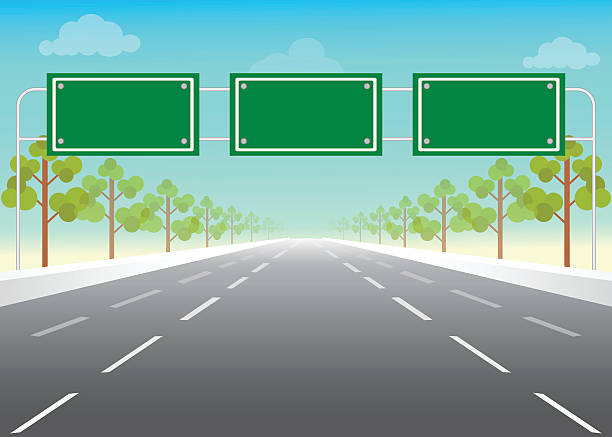
\includegraphics[width=6cm]{pics/multipleLane.jpg}
\end{figure}
  
\end{frame}

\begin{frame}

\frametitle{Ambiguities (cont.)}

\begin{center}
\begin{minipage}{6cm}
\begin{alertblock}{}
``Drive to the person with the dog''
\end{alertblock}
\end{minipage}
\end{center}

\pause
\begin{figure}
\hspace*{-3mm}%
\centering
   
\includegraphics[width=5cm]{pics/personDog.png}
   \pause
   
\includegraphics[width=5cm]{pics/dogCar.png}
\end{figure}
  
\end{frame}

\begin{frame}
\frametitle{Simplified Autonomous Vehicle}
\begin{figure}
\centering
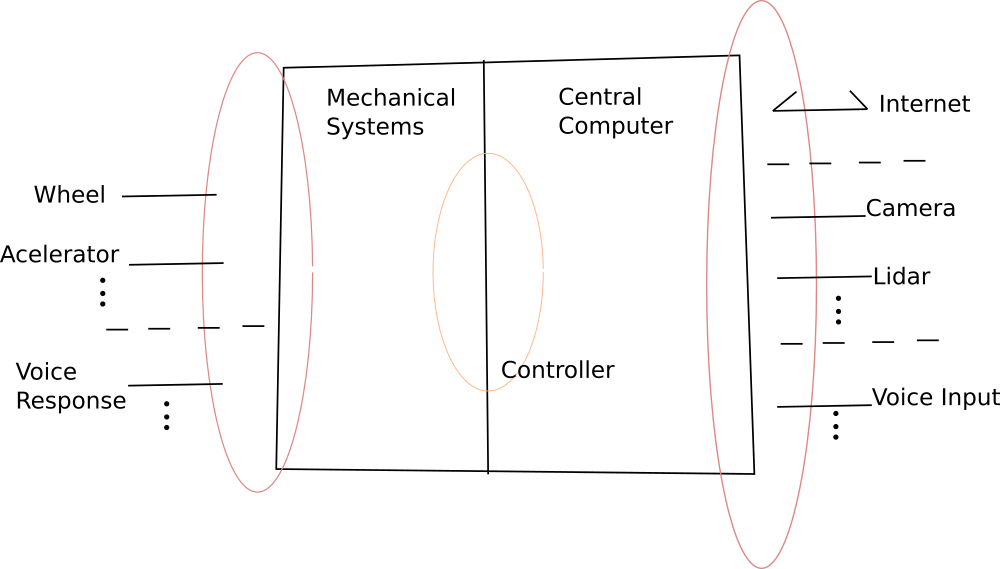
\includegraphics[width=100mm]{pics/selfDriving.png}
\caption{Self-driving car}\label{fig:A1}
\end{figure}

\end{frame}

\begin{frame}
\frametitle{Path}
\begin{figure}
\centering
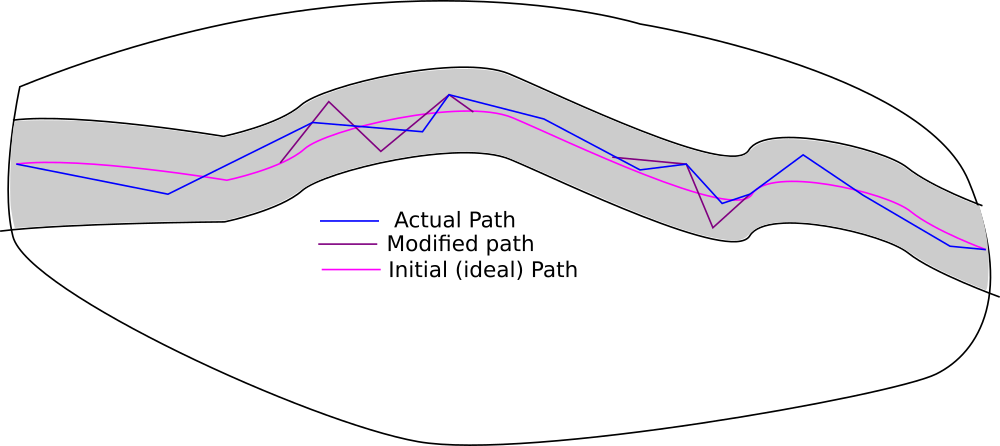
\includegraphics[width=100mm]{pics/diagramTrial1.png}
\caption{Initial, modified, and actual paths/routes}\label{fig:A2}
\end{figure}

\end{frame}

\begin{frame}
\begin{block}{Mathematically Ideal Property}
  $\forall u \in \text{Utt}.\; \exists r \in \text{Routes}$
  such that $\forall r' \in \text{Routes}.\; d(u,r) \leq d(u,r')$
\end{block}
\pause
\begin{exampleblock}{}
where $d$ is some hypothetical metric which should depend on
\pause
\begin{itemize}[<+->]
\item Cost
\item Safety
\item Legality
\item Adversaries
\end{itemize}
\end{exampleblock}
\pause
\begin{exampleblock}{}
and where
\pause
\begin{itemize}[<+->]
\item The set of utterances is a set of strings over a standard alphabet
\item The set of routes is some discretized set of paths in Euclidean 2-space
\end{itemize}
\pause
subject to constraints on the sets imposed by, for example
\pause
\begin{itemize}[<+->]
\item grammars in the case of strings
\item physical objects in the case of paths in Euclidean space
\end{itemize}
\end{exampleblock}



% \begin{itemize}
% \item Functional Programming languages : GF (Grammatical Framework), Haskell, Theorem Provers (Agda, Coq, ...)
% \item Verification for Robotics Systems :  Temporal logic (mostly at the syntactic level, for now)
% \item Natural Language Processing : Semantic Parsing, Controlled Natural Languages
% \end{enumerate}



\end{frame}


\begin{frame}[fragile]
\frametitle{Verification Spectrum}
\begin{figure}
\centering

% https://tikzcd.yichuanshen.de/#N4Igdg9gJgpgziAXAbVABwnAlgFyxMJZABgBpiBdUkANwEMAbAVxiRAB12cYAPHYAMpYwAcwYwABAFEedALZpxAXxBLS6TLnyEUZAIxVajFm1XqQGbHgJEA7KQPV6zVohBmNV7UQBM5Q84mbpzcfIIwOBIQAGbSsgricCpqnlo2KAAs-k7GrhxcvPxCouISAAoAThBoMBU4AJ7J5pZpOsgAbNlGLmwhhcAAshF0aFU1dY0eFprWbWQ+Abm9BWEAqmC4EgAq8DhNqbO+pAs5PcEr-JXVtQ0AtABGdHAwUNu7+9Ne6chZJ91B+VC-AG0BgDAkAGEABYwADGAGthCIPi1DihOn9Ank+mEAJJgbgVOiwvA0SRbGEQCowOTlKpkioombeFB6Y6LM7uFKfVpHADMHIBU1RLOQfPZpyF3JF3yyAsleWFzO+AFYJf9FdLlW1OvKNaYtV82myMoLNc1tUQABykU0Kg2GF4ieBEUDRKpyJBskA4CBIHzc90QT2IPRkH1+0N6QMer1+CNevkx4NerIJ0Mq5MhvSddN6ewgBh0e5gsqWtzCbCwED285A4AAMSYYBJ2kYdIgIiJcjkSIkAihWGie1UFCUQA
% https://tikzcd.yichuanshen.de/#N4Igdg9gJgpgziAXAbVABwnAlgFyxMJZABgBpiBdUkANwEMAbAVxiRAB12cYAPHYAMpYwAcwYwAvp2lde-AKI86AWzTiJICaXSZc+QigCM5KrUYs2nbn0EwcUmbJsQAZg5nWFS1eLgatOth4BEQATCbU9MysiBxO-EKi6o7xwAAKAE4QaDAZOACe-togGEH6RADMEWbRlqkAsnZ0aFk5eYWaxaV6IShkhqZRFrGdgT0GyFUDkeYxIJqmMFAi8ESgLlnKSAAs1DgQSACsEhQSQA
\begin{tikzcd}
\substack{\text{Single}\\\text{Example}} & \substack{\text{Set}\\\text{of}\\\text{Examples}} & \substack{\text{Single}\\\text{Property}} & \substack{\text{Metaproperty}} \\
{} \arrow[rrr, "\text{Verifiability}" description] &                                        &                                & {}                  &    \\
\substack{\text{Unit}\\\text{Testing}} & \substack{\text{Property-based}\\\text{Testing}} & \substack{\text{Model}\\\text{Checking}} & \substack{\text{ITP}} \\

{} \arrow[rd, "FP" description]                    &                                        &                                &                     &    \\
                                                   & {} \arrow[rrr]                         &                                &                     & {}
               
\end{tikzcd}
\end{figure}

\end{frame}

% general
\begin{frame}
\frametitle{Main Idea}

\begin{itemize}[<+->]
\item Functional Programming is all about composition of higher order functions
\item Break down system into composable \emph{big-components}, each of which
\begin{itemize}[<+->]
\item admits composition of \emph{small-components}
\item operates under different verification conditions
\end{itemize}
\item Ensure maps between big-components are functorial with respect to
  small-component composition
\item Verification of system is can similarly be broken into sub-verifications
\end{itemize}
\end{frame}


% more specifically
\begin{frame}
\begin{exampleblock}{More Specifically}
This project contains bits and pieces of :
\end{exampleblock}
\begin{enumerate}
\item Functional Programming Languages : GF (Grammatical Framework), Haskell, Agda
\item Natural Language Processing : Semantic Parsing, Controlled Natural Languages
\item Tools : Grammars, Decidable logics for motion planning and verification
\end{enumerate}
\end{frame}


\begin{frame}
\frametitle{Ideal Pipeline}

\begin{equation} % \label{eq1}
\begin{split}
\text{Utterance} & \mathcolorbox{yellow}{\xrightarrow{\mathit{Speech\ Recognizer}}} \text{String}\\
 & \mathcolorbox{yellow}{\xrightarrow{\mathit{Canonicalization_{LLM}}}} \text{String}\\
 & \xrightarrow{\mathit{Parsing_{GF}}} \text{Abstract Syntax Tree (NL)}\\
 & \xrightarrow{\llbracket - \rrbracket_{Haskell}} \text{Abstract Syntax Tree (LTL)}\\
 & \mathcolorbox{yellow}{\xrightarrow{\vDash_{Agda}}} \text{Verifiable Path}
\end{split}
\end{equation} 
\end{frame}


\begin{frame}
\frametitle{Grammatical Framework}
\begin{itemize}[<+->]
\item Multilingual support
\item Standard Libarary : Resource Grammar Library (RGL)
\item Embedding in Haskell (as GADTs) : Portable Grammar Format (PGF)
\item Simple types, functional programming
\item ``Parallel multiple CFGs''
\item Chomsky Hierarchy : $\text{CFG} < \text{PMCFG} < \text{Context Sensitive Grammar}$
\item Separation of abstract (semantic and syntactic) and concrete (syntactic and
 morphological) considerations
\end{itemize}
\end{frame}

\begin{frame}
\frametitle{Abstract Syntax}
\begin{itemize}[<+->]
\item Semantic considerations
\item Coarse meaning space
\item Tree formation
\item Categories cat (basic types)
\item Named function fun of arbitrary arities over them
\end{itemize}
\end{frame}

\begin{frame}
\frametitle{Concrete Syntax}
\begin{itemize}[<+->]
\item Lexical Details
\item Function body, how strings are formed
\item 
\end{itemize}
\end{frame}

\begin{frame}[fragile]
\frametitle{TOUCHDOWN Dataset}
\fontsize{9pt}{10pt}\selectfont

\begin{verbatim}
([(["Go"],5527),(["be"],5300),(["turn"],4154),(["Turn"],4154)],["VB"])
([(["left"],228),(["came"],59),(["made"],47),(["started"],44)],["VBD"])
([(["going"],1684),(["facing"],939),(["moving"],849),(["passing"],617)],["VBG"])
([(["left"],1733),(["parked"],616),(["painted"],307),(["fenced"],263)],["VBN"])
([(["are"],3554),(["'re"],1185),(["reach"],1100),(["get"],770)],["VBP"])
([(["is"],4919),(["has"],795),(["'s"],471),(["ends"],93)],["VBZ"])
\end{verbatim}

n-grams : the 9-gram ``so you are moving with the flow of traffic'' occurs 311

\end{frame}



\begin{frame}[fragile]
\frametitle{Ontological Categories}
\begin{verbatim}
  cat
    PosCommand   ; -- go to the store
    Place        ; -- the store
    Time         ; -- in 5 minutes
    Action       ; -- drive
    Way          ; -- to
    How          ; -- quickly
    Where        ; -- left
    AdvPh        ; -- to the store
    UndetObj     ; -- store
    Determ       ; -- the
    Object       ; -- the store
    Number       ; -- a
    Conjunct     ; -- and
    Condition    ; -- there is a museum
    Descript     ; -- big
\end{verbatim}
\end{frame}

\begin{frame}[fragile]
\frametitle{GF Functions}
\begin{verbatim}
fun
  -- Explicit Temporality
  DoTil     : Action -> Time -> PosCommand ; go in one minute

  -- Modified action
  ModAction : Action -> AdvPh -> Action ; -- go to the store

  -- Adverbial Phrases
  MkAdvPh     : Way   -> Object -> AdvPh ; -- to the store

  -- Noun Phrases
  WhichObject : Determ -> UndetObj -> Object ; -- the red dog

  -- Modified Noun
  ModObj : Descript -> UndetObj -> UndetObj ; -- black dog
\end{verbatim}
\end{frame}

\begin{frame}[fragile]
\frametitle{Base Ingredients}

These represent the tree leaves to be grounded!

\begin{verbatim}
fun
  Quickly : How      ;
  Left    : Where    ;
  To      : Way      ;
  After   : Way      ;
  Store   : UndetObj ;
  Traffic : UndetObj ;
  London  : Place    ;
  Drive   : Action   ;
  Turn    : Action   ;
  Big     : Descript ;
  A       : Determ   ;
\end{verbatim}
\end{frame}


\begin{frame}
\fontsize{9pt}{10pt}\selectfont
\begin{exampleblock}{}
go to the store, turn left and stop at the woman with the dog. go to the bridge. finish.
\end{exampleblock}

\begin{figure}

\centering
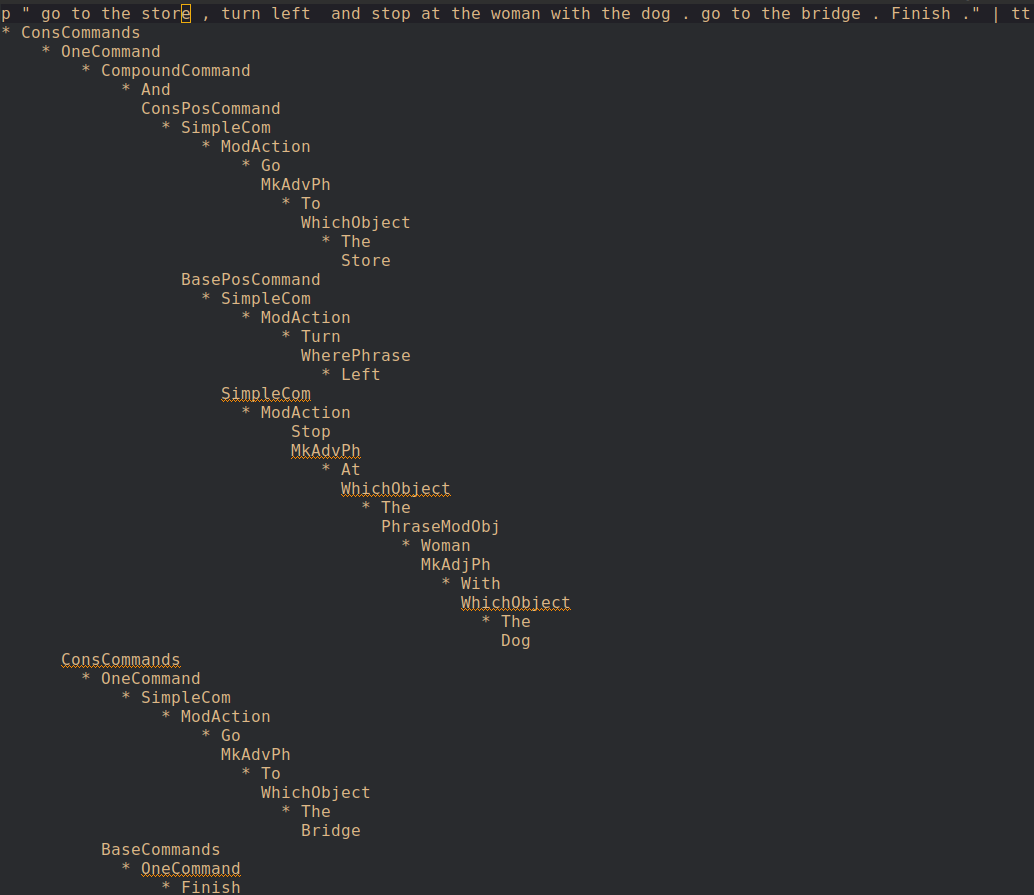
\includegraphics[width=90mm]{pics/wholeAST.png}
\end{figure}
\end{frame}

\begin{frame}
\fontsize{9pt}{10pt}\selectfont
\begin{exampleblock}{}
go to the store, turn left and stop at the woman with the dog. go to the bridge. finish.
\end{exampleblock}

\begin{figure}

\centering
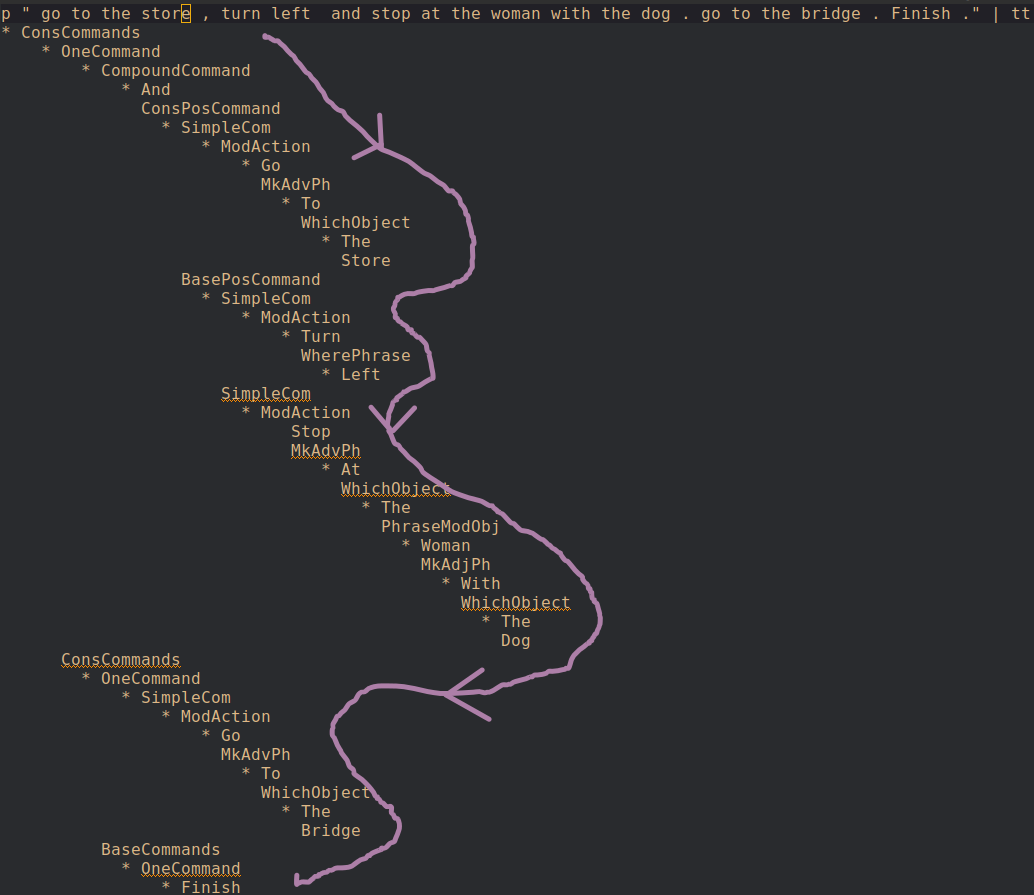
\includegraphics[width=90mm]{pics/WithArrow.png}
\end{figure}
\end{frame}

% the more "kinds" of branching there are, the more complicated
% can the different kinds of branching interact : this syntactic question
% manifests as a semantic one


\begin{frame}
\fontsize{9pt}{10pt}\selectfont
\begin{exampleblock}{}
go to the store, turn left and stop at the woman with the dog. go to the bridge.
finish.
\end{exampleblock}

\begin{figure}

\centering
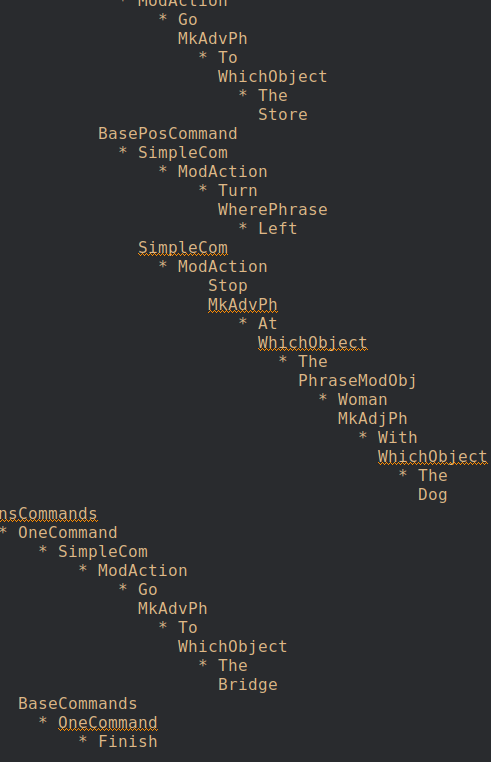
\includegraphics[width=50mm]{pics/zoomedScreenshot.png}
\end{figure}
\end{frame}

\begin{frame}
\fontsize{9pt}{10pt}\selectfont
\begin{exampleblock}{}
go to the store, turn left and stop at the woman with the dog. go to the bridge.
finish.
\end{exampleblock}

\begin{figure}

\centering
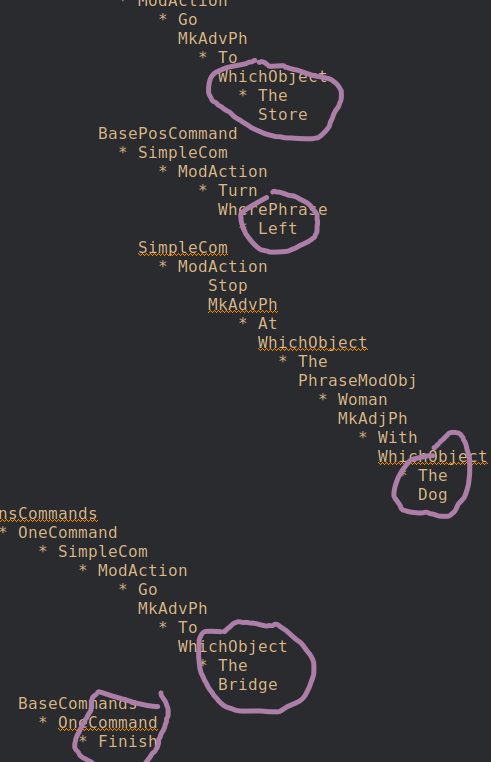
\includegraphics[width=50mm]{pics/circledZoom.png}
\end{figure}
\end{frame}


\begin{frame}[fragile]
\begin{exampleblock}{Alternative Interpretation}
go (to the store, turn left and stop (at the woman)) with the dog. 
\end{exampleblock}
\pause
\begin{verbatim}
ModAction
  * Stop
    MkAdvPh
      * At
        WhichObject
          * The
            Woman
MkAdvPh
  * With
    WhichObject
      * The
        Dog
\end{verbatim}
\pause
\begin{alertblock}{}
Need a temporal until operator, $U$, to construct a semantically justifiable interpretation
\end{alertblock}
\end{frame}


\begin{frame}[fragile]
\frametitle{Haskell LTL}

\fontsize{9pt}{10pt}\selectfont
\begin{exampleblock}{}
go to the store, turn left and stop at the woman with the dog. go to the bridge.
finish.
\end{exampleblock}

\begin{verbatim}
  F (Meet
      (Atom "the_store")
      (F (Meet
          (Atom "turn_left")
          (F (Meet
               (Atom "the_woman_with_the_dog")
               (F (Meet
                    (Atom "the_bridge")
                    (G (Atom "FINISHED")))))))))
\end{verbatim}
\end{frame}

\begin{frame}[fragile]
\frametitle{Haskell Semantics}
\fontsize{9pt}{10pt}\selectfont
\begin{block}{}
Sequence of future states reveal a simple list flattening procedure which
amounts to an exceedingly simple denotational semantics
\end{block}
\pause
\begin{verbatim}
semantics :: GListCommands -> Phi
semantics x =
  let (GListCommands ((GOneCommand y) : _)) = normalizeList x
  in case y of
      q@(GSimpleCom a) -> astToAtom q
      (GCompoundCommand GAnd (GListPosCommand xs)) -> listCommand2LTL xs
\end{verbatim}
\pause
\begin{verbatim}
normalizeList ::  GListCommands -> GListCommands
  where
    normalizeNestedLists :: GListCommands -> GListPosCommand
      where
        normalizeListPosCommand :: GListPosCommand -> GListPosCommand
          where
            unSentence :: [GCommands] -> [GPosCommand]
            flattenSublist :: GPosCommand -> [GPosCommand]
            where
              getListPosCommands :: GListPosCommand -> [GPosCommand]
\end{verbatim}
\end{frame}





\begin{frame}
\frametitle{Linear Temporal Logic}
\begin{itemize}
\item Modal logic (temporal modality)
\item Allows one to reason about sequential actions
\item Verification for robotics systems
\item Objective in reinforcement learning
\item Other temporal logics (Signal TL, Computation Tree Logic, ...)
\item Decidable 
\end{itemize}

\begin{block}{Complexity (and expressivity)}
$\text{Propositional Logic} < \text{Temporal Logic} <_{undecidable} \text{First Order Logic}$
\end{block}

\begin{exampleblock}{Temporal Operators}
\begin{itemize}
\item $X \phi$ : in the next state, phi holds
\item $\diamond \phi$ : exists a future state such that $\phi$ holds ($F \phi$)
\item $\square \phi$ : $\phi$ holds for every future state ($G \phi$)
\end{itemize}
\end{exampleblock}

\end{frame}


\begin{frame}
\begin{exampleblock}{}
This project is quite multifaceted, still in a somewhat primordial state (and therefore may be taken in many directions).
\end{exampleblock}

\begin{block}{}
Goal : Design a controlled natural language which is 
\end{block}

\begin{itemize}
\item Suitable as an ``approximation'' for a voice assistant for an autonomous vehicle
\item Has a well defined semantics in temporal logic
\item Seeking to balance breadth and depth of our system
\end{itemize}
\end{frame}



\begin{frame}
\frametitle{Trade-offs}
\begin{itemize}[<+->]
\item Depth versus breadth
\begin{itemize}[<+->]
\item Breadth : Wide coverage, usable by non-experts (where ML comes in)
\item Depth   : Well-behaved, verifiable (where FP comes in)
\end{itemize}
\item Specificity and generality
\item Formality and formalizability
\item Verifiability and validity
\end{itemize}
\end{frame}


\begin{frame}
\frametitle{Where does ML come in?}

\begin{exampleblock}{Language Models}
\begin{itemize}
\item Foundation models - future of NLP?
\item BERT, GPT3, ...
\item Pretrain and then fine-tune
\end{itemize}
\end{exampleblock}

\begin{block}{Ingredients}
\begin{itemize}
\item Semantic Parser : NL Utterance -> Formal Language form
\item Touchdown Data Set : ~13000 sequences
\item Few-shot semantic parsers paper (Microsoft Research) - open source Pytorch code
\end{itemize}
\end{block}

\begin{alertblock}{Idea}
Integrate their technique and code with our parser and dataset
\end{alertblock}

\end{frame}


\begin{frame}
\frametitle{}
\begin{figure}
\hspace*{-3mm}%
   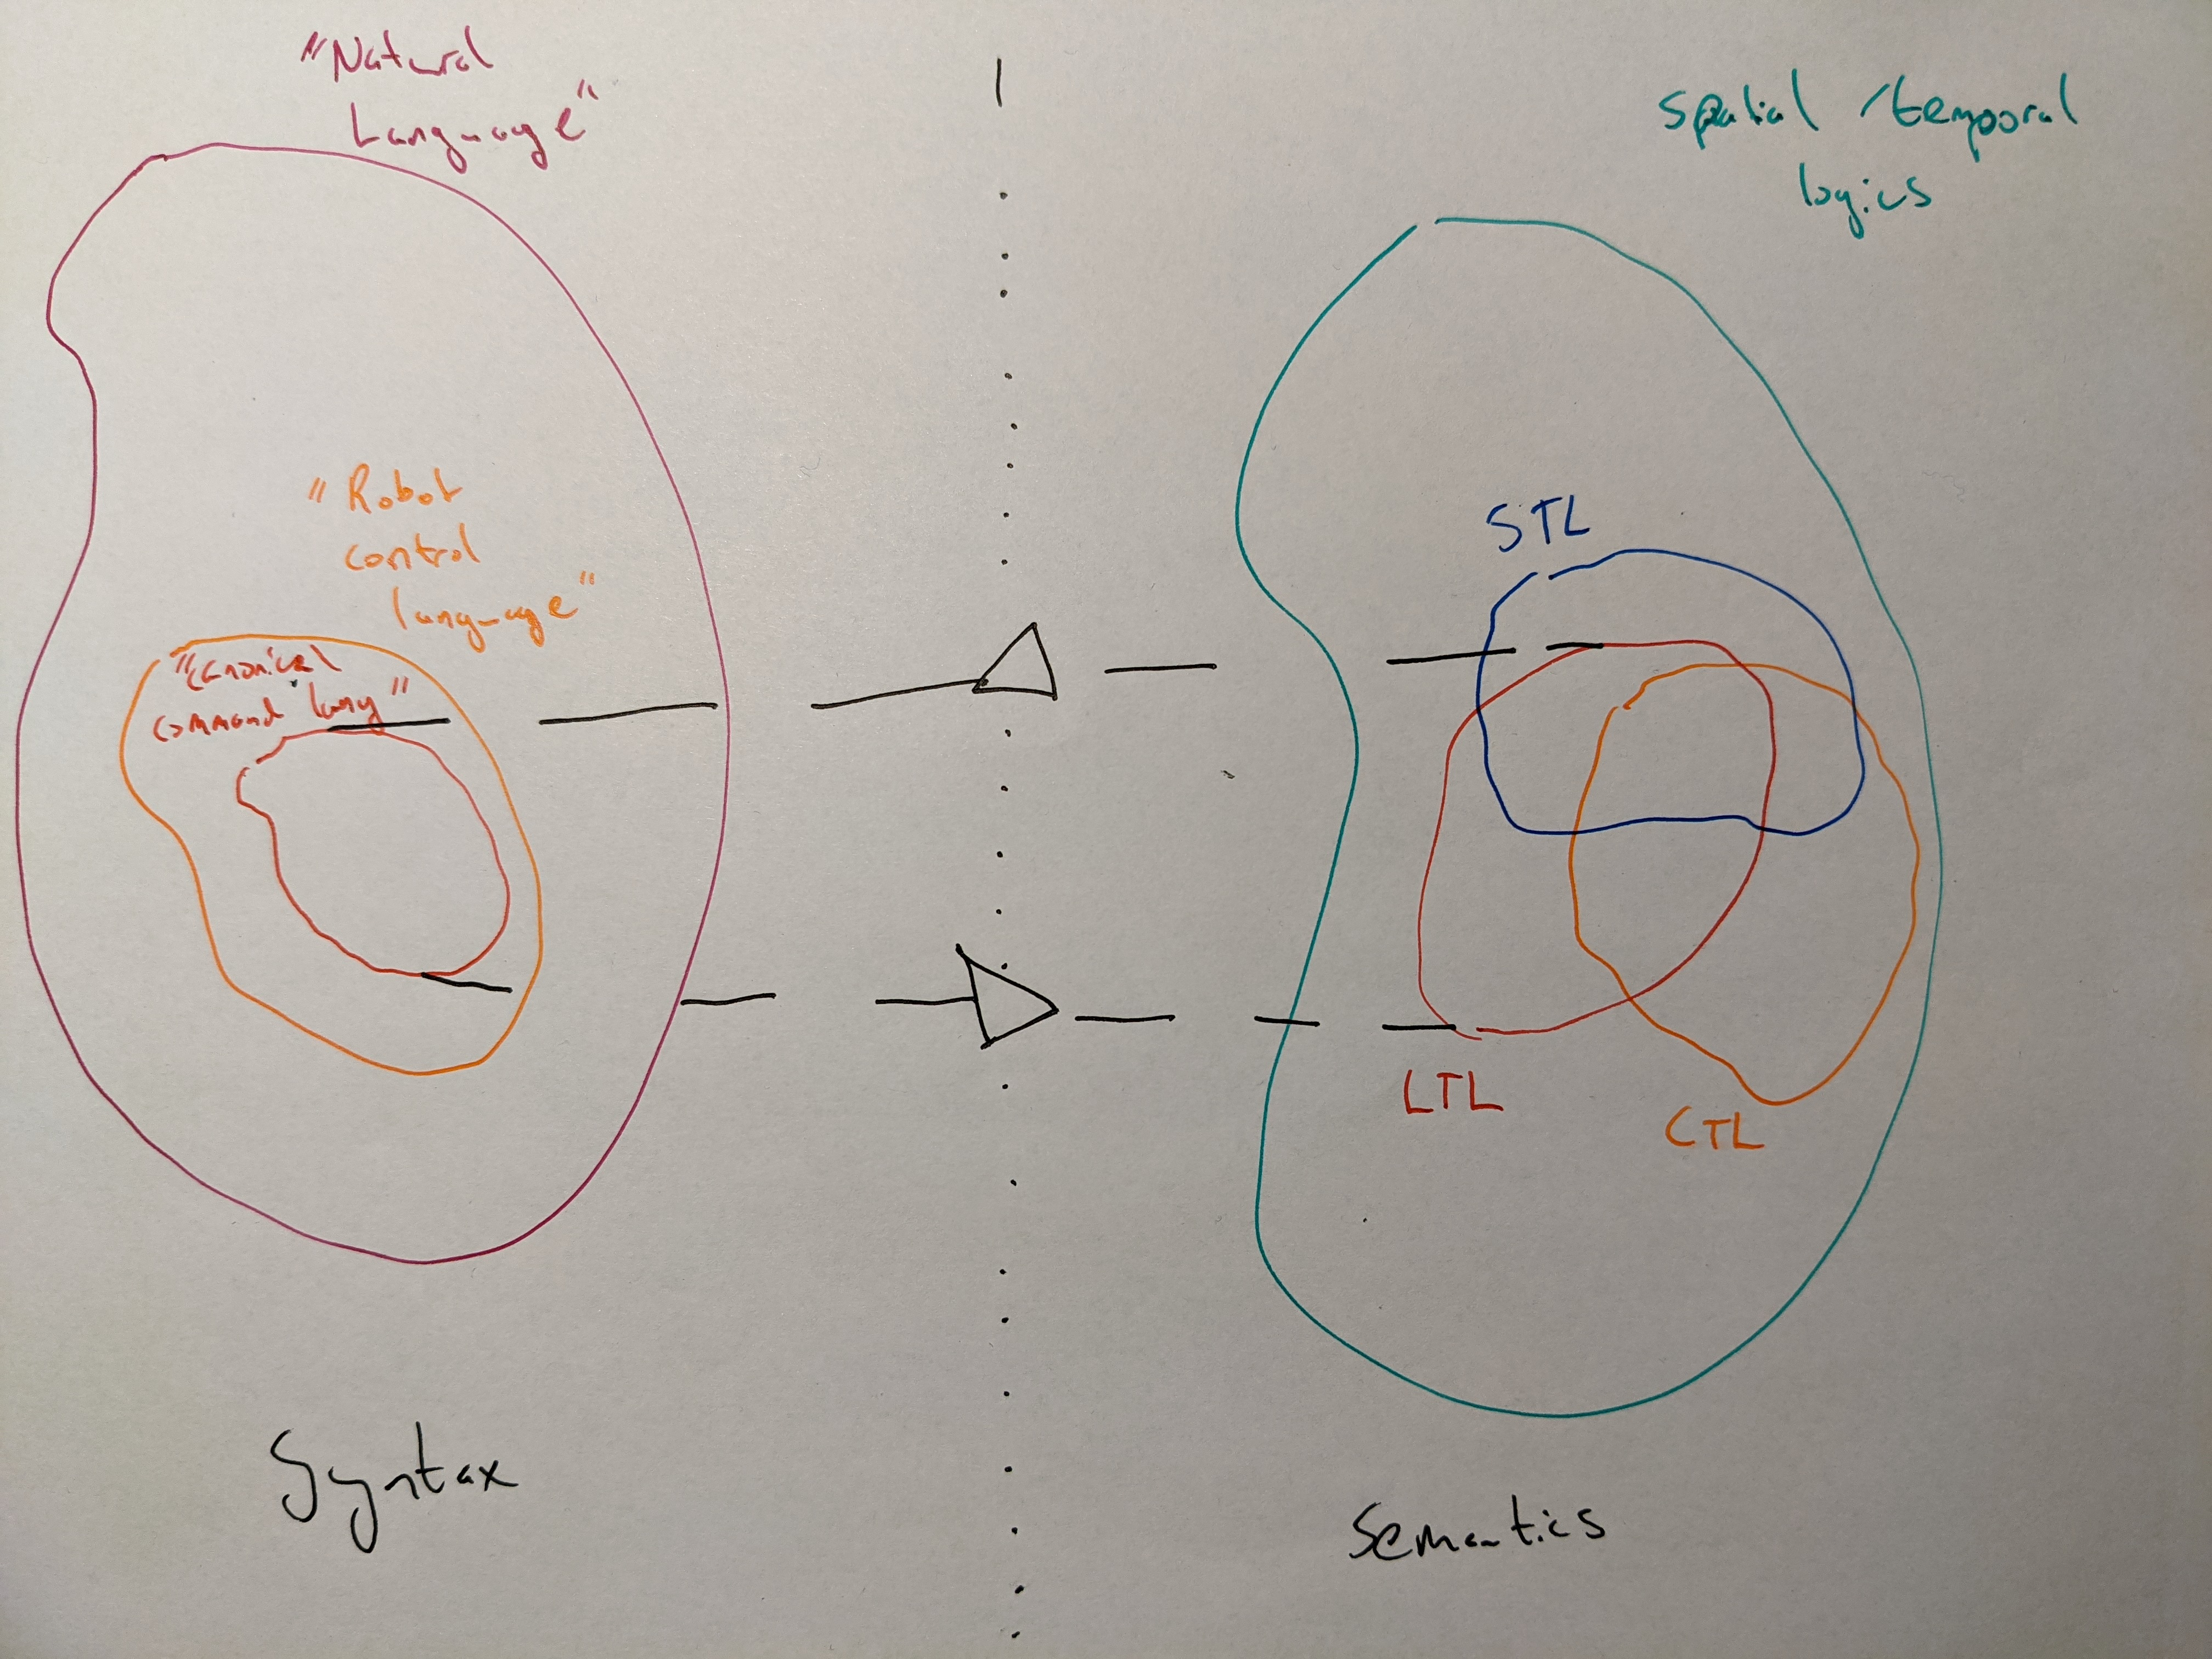
\includegraphics[width= \paperwidth]{pics/one.jpg}
\end{figure}
\end{frame}

\begin{frame}
\frametitle{}
\begin{figure}
\hspace*{-3mm}%
   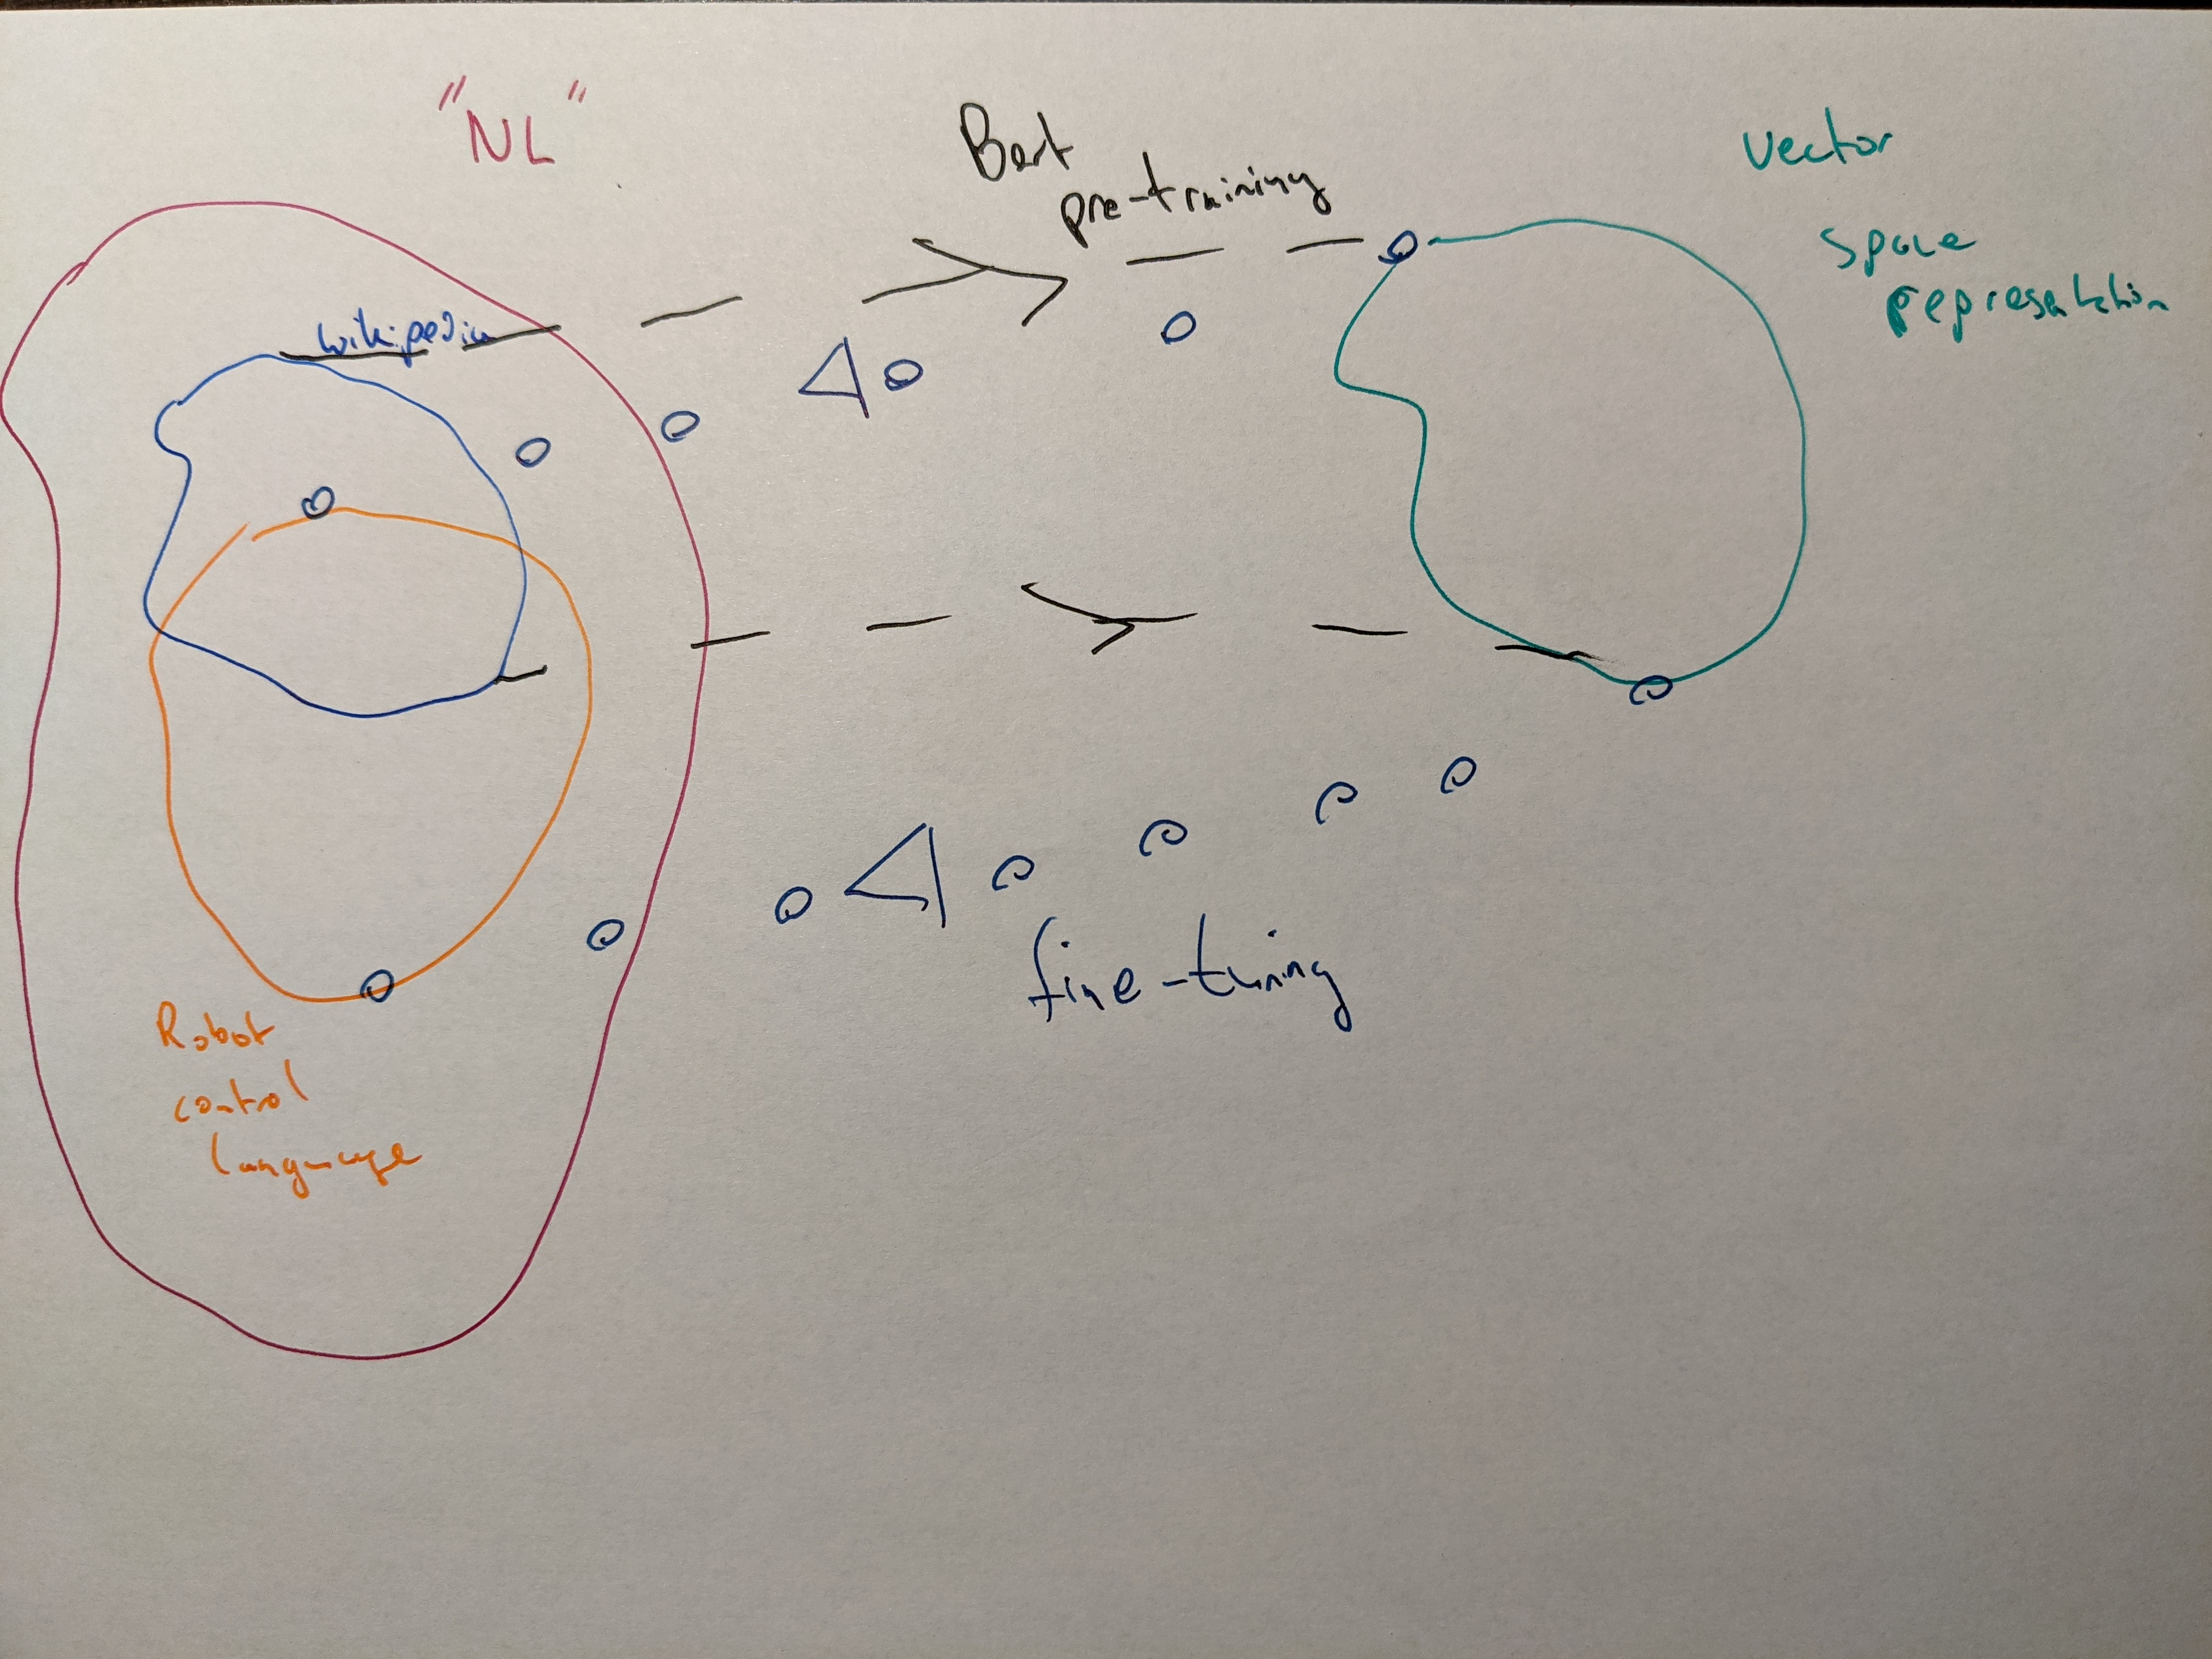
\includegraphics[width= \paperwidth]{pics/two.jpg}
\end{figure}
\end{frame}


\begin{frame}
\frametitle{}
\begin{figure}
\hspace*{-3mm}%
   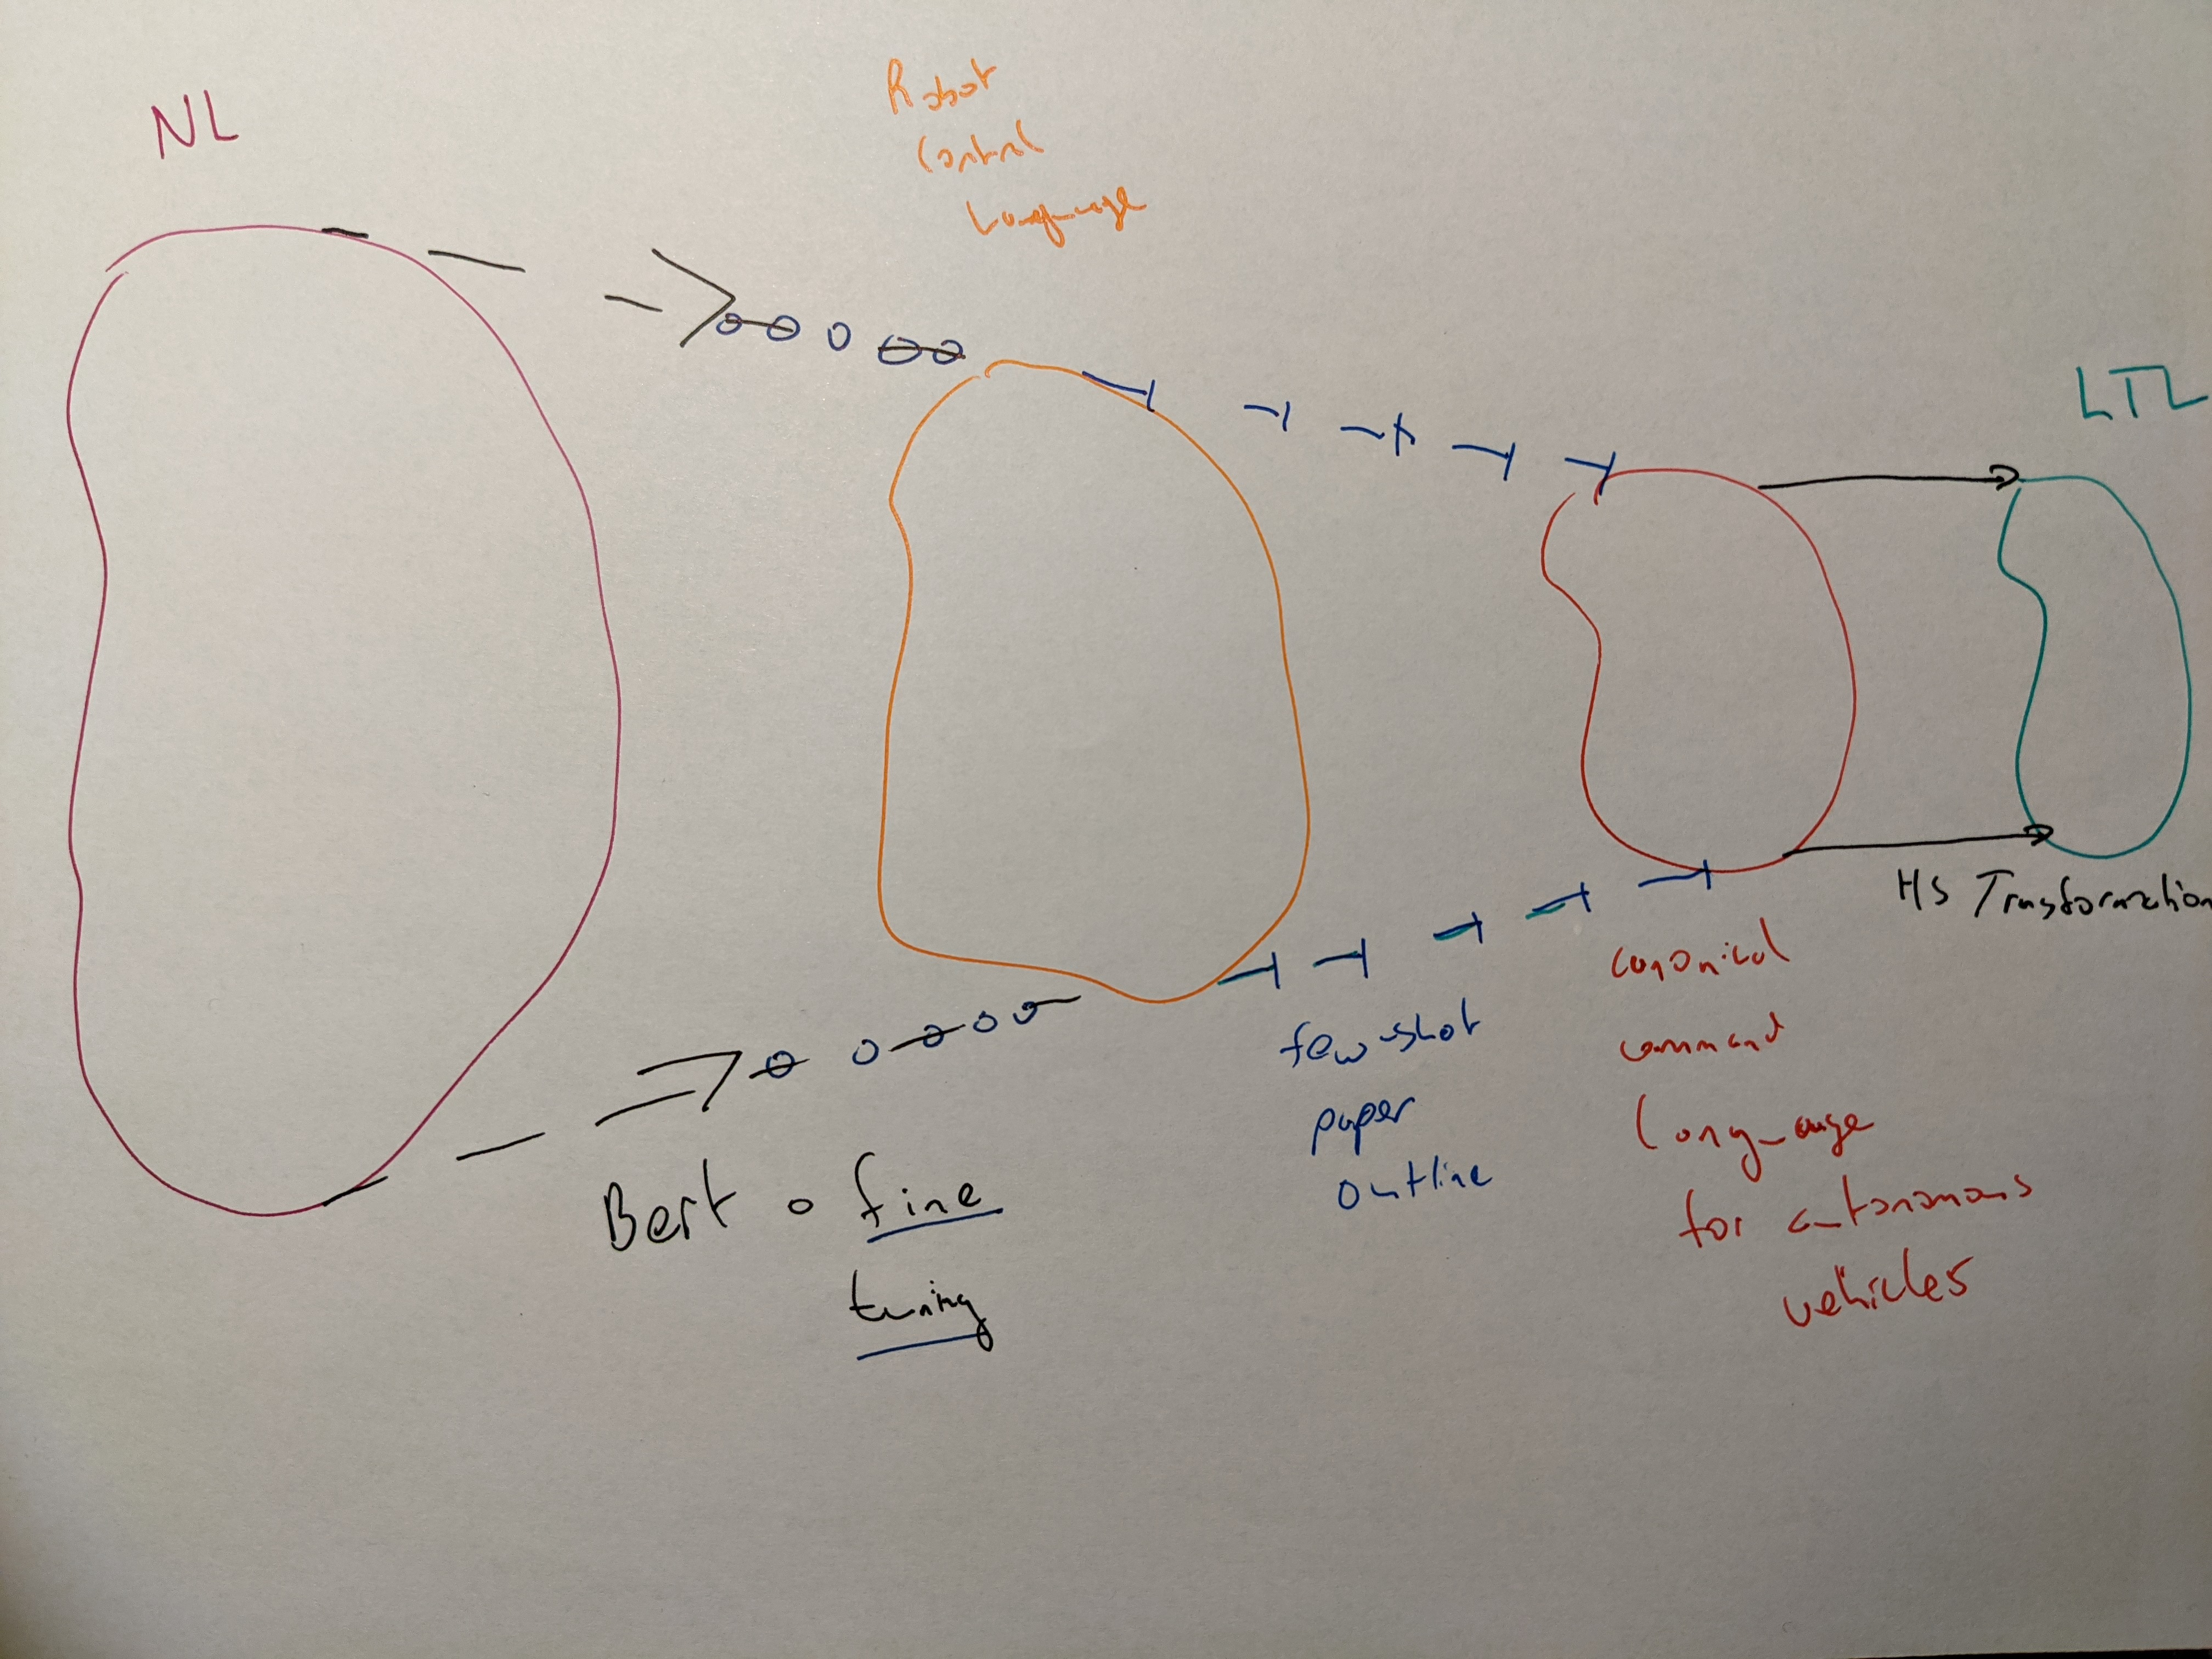
\includegraphics[width= \paperwidth]{pics/three.jpg}
\end{figure}
\end{frame}

\begin{frame}
\frametitle{Future}

\begin{itemize} 
\item Expand parser itself
\item Work on semantics , more expressive logic, etc
\item Ground semantics to Touchdown location map
\item Better data set?
\item Working on a draft document, with references, of everything shown here.
\end{itemize} 

\end{frame}

\begin{frame}
Acknolwedgements
\end{frame}

\end{document}
